\documentclass[tikz, border = 2pt]{standalone}

%---------------------------------------------------------------------------%
% PACKAGES                                                                  %
%---------------------------------------------------------------------------%

%----- MATH
%---------------------------------------------------------------------------%
\usepackage{amsmath, amssymb}

%----- FIGURES
%---------------------------------------------------------------------------%
\usepackage{color}
\usepackage{pgfplots}
\pgfplotsset{compat=1.13}

%---------------------------------------------------------------------------%
%                                MINES COLORS                               %
%---------------------------------------------------------------------------%

%---------- OFFICIAL COLORS
\definecolor{MPTblue}{RGB}{0,94,158}

\begin{document}

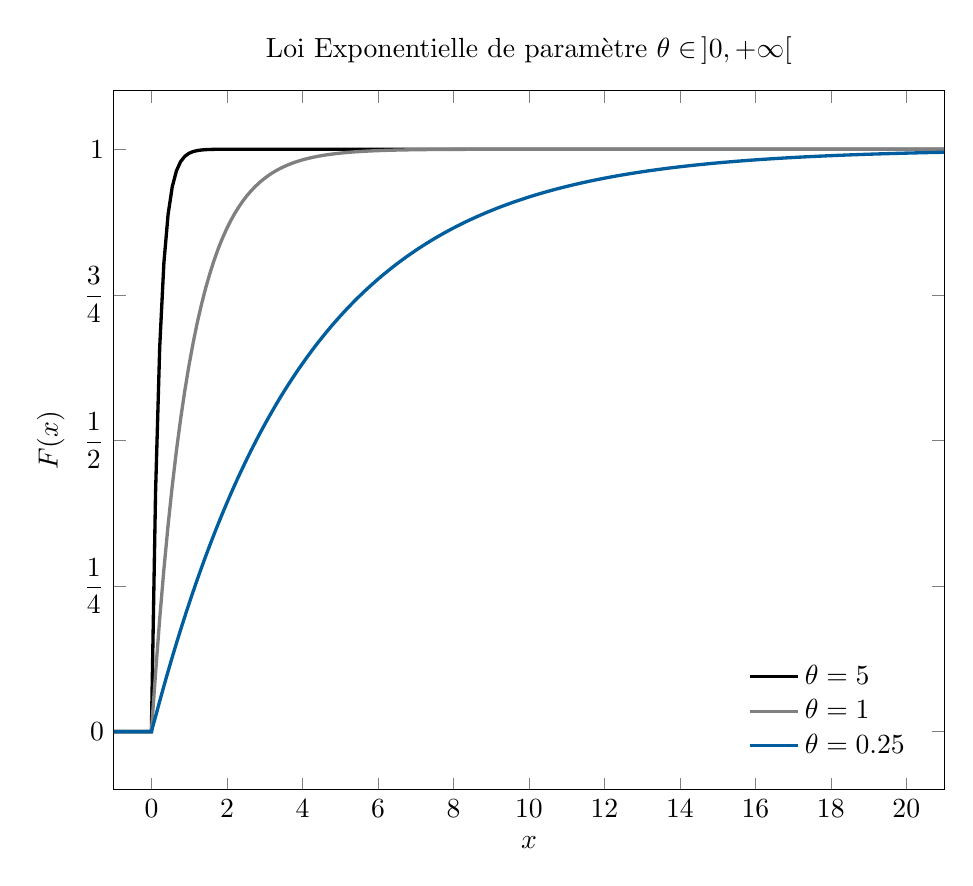
\begin{tikzpicture}
\begin{axis}[width = \textwidth,
title style = {align = center},
title={Loi Exponentielle de param\`etre $\theta \in\, ]0,+\infty[$},
xlabel={$x$},
ylabel={$F(x)$},
legend pos = south east,
legend style = {draw=none},
legend cell align = left,
xmin = -1,
xmax = 21,
ytick = {0,0.25,0.5,0.75,1},
yticklabels = {$0$, $\dfrac{1}{4}$, $\dfrac{1}{2}$, $\dfrac{3}{4}$, $1$},
ylabel near ticks,
domain = -1:21
]
\addplot[black, very thick, samples = 200] {(1 - exp(-5*x))*(x>=0)};
%
\addplot[black!50, very thick, samples = 200] {(1 - exp(-x))*(x>=0)};
%
\addplot[MPTblue, very thick, samples = 200] {(1 - exp(-x/4))*(x>=0)};
%
\legend{{$\theta = 5$},{$\theta = 1$},{$\theta = 0.25$}}
\end{axis}
\end{tikzpicture}

\end{document}